\section{Mobile Manipulator [25 pts]}

You can use MATLAB or Python for this exercise. The robot in Figure~\ref{fig:Mobile Manipulator} is given: 2WD mobile robot with attached a planar serial manipulator. On the serial manipulator, each link is connected via a revolute (rotational) joint, except for the end-effector (the gripper), which is fixed to the final link. Given this robot: 

\begin{enumerate}[(a)]
    \item Write the transformation matrices between subsequent reference frames, starting from the end-effector frame $\{e\}$ $(G^2_E,G^1_2,...,G^s_B)$, and compute the transformation matrix from the end-effector frame $\{E\}$ to the global frame $\{s\}$. Report the symbolic forms of these matrices in full (report simplified versions when possible, with MATLAB you can simplify with simplify(expression)) [12 pts]
    \item At the following configuration of the robot:
    \begin{equation*}
        \theta=-\frac{\pi}{2}, \alpha=\frac{\pi}{6}, \gamma=\frac{\pi}{4}, l_1=l_2=1, l_B=0.5, x=y=0.8
    \end{equation*}
    What are the coordinates of these points in the spatial frame $\{s\}$? $p^E_1=\begin{bmatrix}
        0\\0
    \end{bmatrix},p^E_2=\begin{bmatrix}
        0.5\\1
    \end{bmatrix}$ [5 pts]
    \item Suppose that a point $q^B=\begin{bmatrix}
        1\\2
    \end{bmatrix}$ is measured in the reference frame $\{B\}$, and the objective is for the robot arm to reach and grasp and object at this location. The movement of the robot for grasping is relative to the end-effector frame. With the configuration at point (b) and using the transformation matrices obtained in (a), compute the coordinates of this point in the frame $\{E\}$. 
    Report the procedure and the final coordinates, no need to report the full symbolic equations at each step. [8 pts]

\end{enumerate}

\begin{figure}[h!]
    \centering
    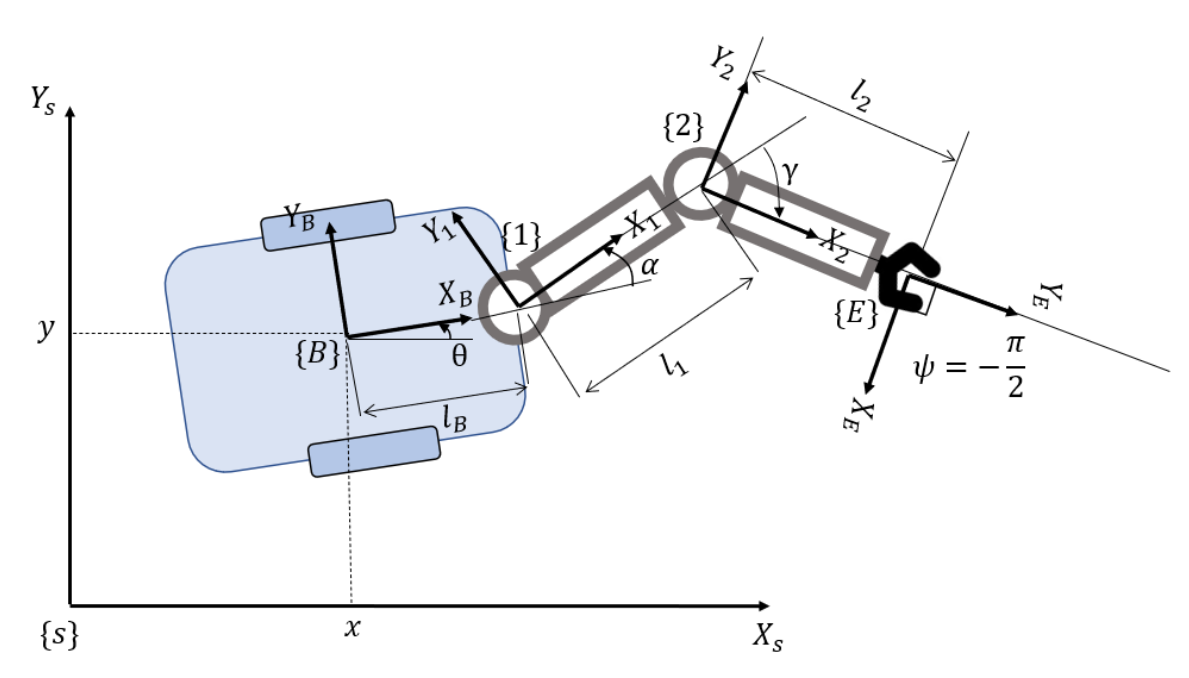
\includegraphics[width=0.7\textwidth]{img/mobile_manipulator.png}
    \caption{Mobile robot with plannar serial manipulator}
    \label{fig:Mobile Manipulator}
\end{figure}
